% !TeX root = main.tex
\chapter{Results and Discussion}
\section{Kinematic control}
\subsection{The target curve}
The considered curve $\mathcal{C}$ was based on the hyperbolic paraboloid while rotating in the $x$ axis in the world frame. Its parametrization is expressed as 
\begin{align}
    \mathbf{H}_d(s) = \begin{bmatrix}
        1 & \ \ 0 & 0 & rc_\theta\\
        0 & \ \ c_\theta & s_\theta & rs_\theta\\
        0 & -s_\theta & c_\theta & b + dr^2(c_\theta^2 - s_\theta^2)\\
        0 & \ \ 0 & 0 & 1
    \end{bmatrix},
\end{align}
where $c_\theta$ and $s_\theta$ denotes $\cos\theta$ and $\sin\theta$ respectively, $\theta = 2\pi s$, $b=\qty{1}{\meter}$, $d=\qty{0.2}{\meter}$, and $r=\qty{1}{\meter}$.

\subsection{The choice of S map}
Let $\boldsymbol{\xi} = [\xi_1 \ \xi_2 \ \xi_3 \ \xi_4 \ \xi_5 \ \xi_6]^\top$. The map $\SL$ used is:
\begin{equation}
    \SL[\boldsymbol{\xi}] = \left[\begin{array}{cccc} 
    \ 0 & -\xi_6 & \ \ \xi_5 & \ \ \xi_1 \\
    \ \ \xi_6 & \ 0 & -\xi_4 & \ \ \xi_2 \\
    -\xi_5 & \ \ \xi_4 & \ 0 & \ \ \xi_3 \\
    \ 0 & \ 0 & \ 0 & \ 0
    \end{array}\right].
\end{equation}
The basis $\mathbf{E}_1, ... ,\mathbf{E}_6$ of the Lie algebra $\mathfrak{se}(3)$ can be obtained by $\mathbf{E}_k = \SL[\mathbf{e}_k]$, where $\mathbf{e}_k$ are the columns of the $6 \times 6$ identity matrix. Geometrically, the interpretation for this choice of basis is that $\boldsymbol{\xi}$ is the classical \emph{twist} in mechanics. More precisely, $\boldsymbol{\omega} \triangleq [\xi_4 \  \xi_5 \  \xi_6]^\top$ represents the $x$, $y$ and $z$ components of the angular  velocity  measured in the fixed frame, whereas $\mathbf{v} \triangleq [\xi_1 \  \xi_2 \  \xi_3]^\top$ represents the $x, y$ and $z$ velocities of the virtual point at the origin of the fixed frame, measured in this fixed frame. This is related to the object's linear velocity $\dot{\mathbf{p}}$  by $\dot{\mathbf{p}} = \boldsymbol{\omega} \times \mathbf{p} + \mathbf{v}$.

\subsection{Parameters}
The optimization problem in \eqref{eq:optimization-problem-distance-definition-point-curve} was solved by discretizing the curve $\mathcal{C}$ using $\num{5000}$ points and determining the optimal $s=s^*$ through a brute-force approach. This discretization was also used to compute $\frac{d}{ds}\mathbf{H}_d(s)$ using finite differences, which is necessary for implementing $\boldsymbol{\xi}_T = \SL^{-1}(\frac{d\mathbf{H}_d}{ds}(s^*)\mathbf{H}_d(s^*)^{-1})$. The chosen gains were $k_N(D) = \tanh(20D)$ and $k_T(D) = 1 - 0.5\tanh(D)$. The system was simulated for $\qty{15}{\second}$ using the approximation $\mathbf{H}(t+\Delta t)\approx \exp(\SL[\boldsymbol{\Psi}]\Delta t)\mathbf{H}(t)$, with a time step of $\Delta t=\qty{0.01}{\second}$. The initial condition $\mathbf{H}(0)$was set as follows:
\begin{align}
    \mathbf{H}(0) = \begin{bmatrix}
        \frac{\sqrt{2}}{2} & -\frac{\sqrt{2}}{2} & 0 & -2\\
        \frac{\sqrt{2}}{2} & \ \frac{\sqrt{2}}{2} & 0 & -1\\
        0 & \ 0 & 1 & \ \ 0\\
        0 & \ 0 & 0 & \ 1
    \end{bmatrix}.
\end{align}

\subsection{Results}
\begin{figure}[ht!]
    \centering
    % First subfigure
    \begin{subfigure}[b]{0.32\textwidth}
        \centering
        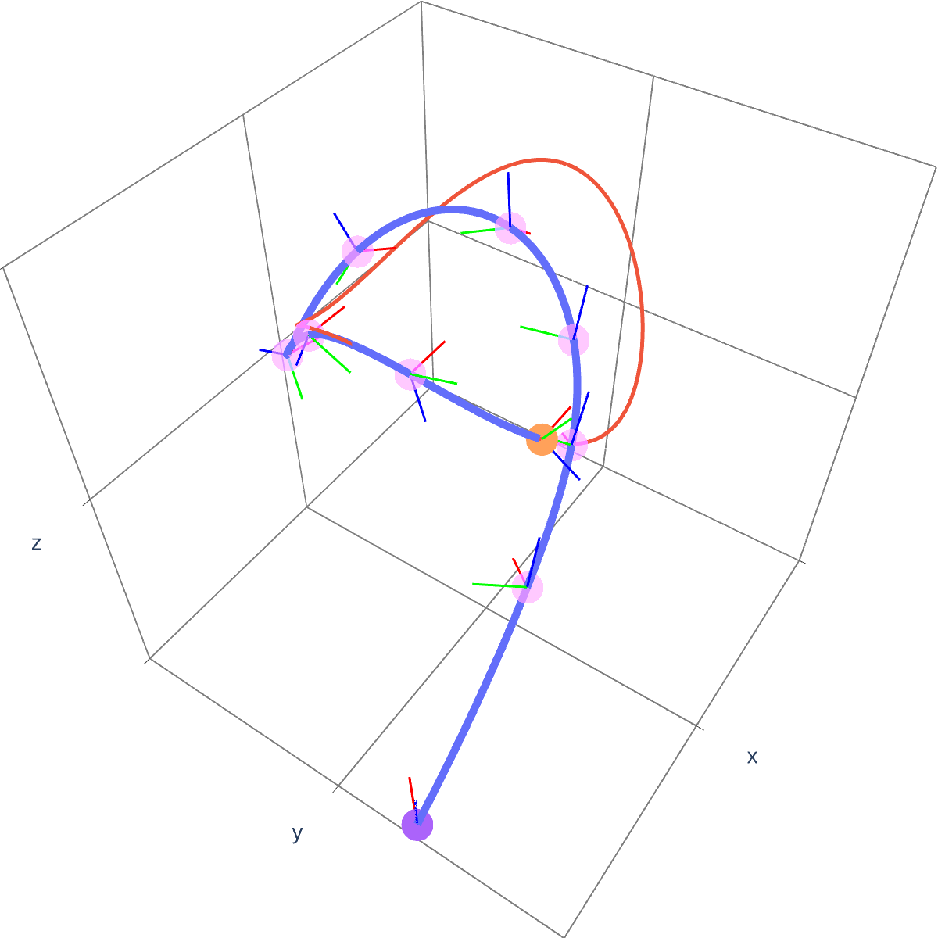
\includegraphics[width=\textwidth]{figures/vf_automatica_1.pdf} % Replace with your image
        \caption{$t\in[0, 5]s$}
        \label{fig:vfplot-first}
    \end{subfigure}
    \hfill
    % Second subfigure
    \begin{subfigure}[b]{0.32\textwidth}
        \centering
        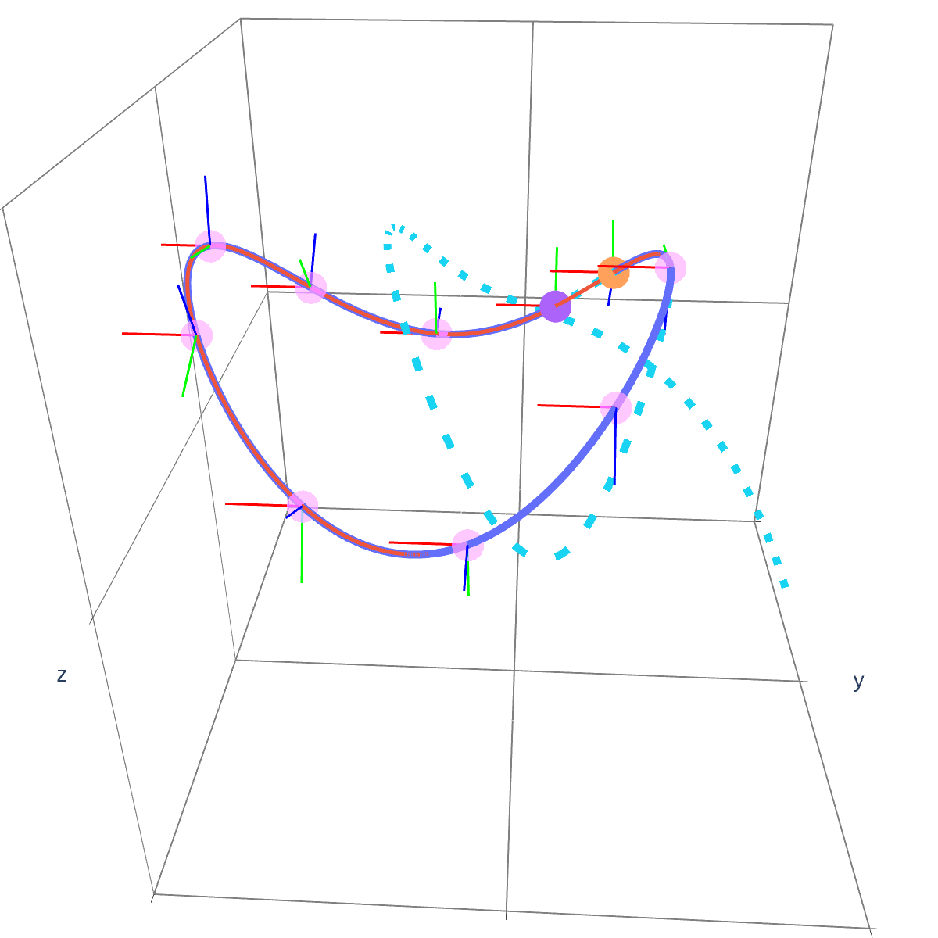
\includegraphics[width=\textwidth]{figures/vf_automatica_2.pdf} % Replace with your image
        \caption{$t\in[5, 9.7]s$}
        \label{fig:vfplot-second}
    \end{subfigure}
    \hfill
    % Third subfigure
    \begin{subfigure}[b]{0.32\textwidth}
        \centering
        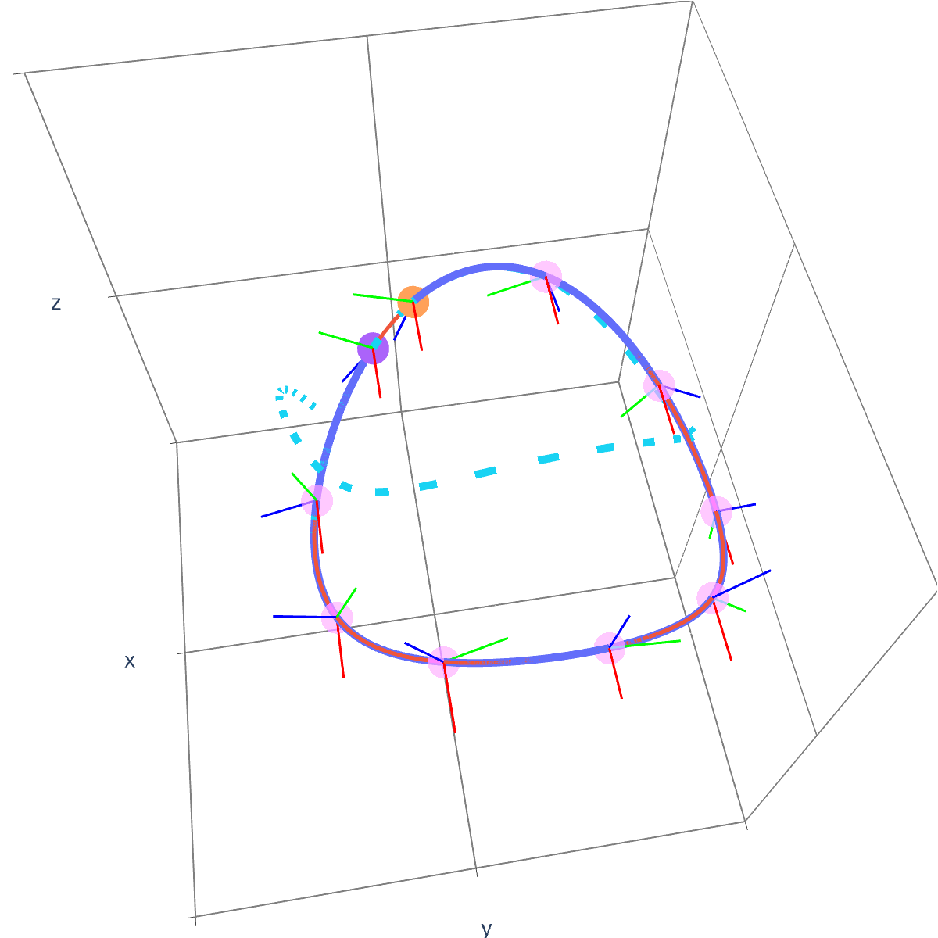
\includegraphics[width=\textwidth]{figures/vf_automatica_3.pdf} % Replace with your image
        \caption{$t\in[9.7, 14.5]s$}
        \label{fig:vfplot-third}
    \end{subfigure}
    \caption{The solid blue line depicts the system trajectory, while the solid red line indicates the target curve. The dashed light blue line represents the past trajectory. The initial and final positions are marked by purple and orange spheres, respectively. Translucent pink spheres denote intermediary positions, with orientation frames shown by RGB axes.}
    \label{fig:vfplot-trajectory}
\end{figure}
\begin{figure}[ht!]
    \centering
    \def\svgwidth{.8\linewidth}
    {\tiny\import{figures/}{distance_pos_ori_D.pdf_tex}}
    \caption{Value of EC-distance $D$, position error in centimeters and orientation error in degrees along time.}
    \label{fig:position-orientation-errors}
\end{figure}
We implemented the code in C++. On average, the computation of the vector field took $60\pm5$ milliseconds per iteration on a single core of an Intel i5-10300H @ 4.5GHz CPU, with 8 GB of RAM. On average, $99.5\%$ of this time was spent solving the optimization problem in \eqref{eq:optimization-problem-distance-definition-point-curve}. Since the optimization process is highly parallelizable -- allowing for the simultaneous computation of $\widehat{D}(\mathbf{H},\mathbf{H}_d(s))$ across different discretized $s$ -- the computational effort could be significantly reduced by leveraging parallel architectures such as GPUs, SIMD, or multi-threading. The system's trajectory is illustrated in \cref{fig:vfplot-trajectory}, while the values of the distance function $D$ are shown in \cref{fig:position-orientation-errors}. Additionally, \cref{fig:position-orientation-errors} provides a more intuitive representation of the position error (in centimeters) and the orientation error (in degrees). The results confirm that the system successfully converges to the desired curve and circulates around it as expected. Once the system reaches the curve, it remains there without deviation. Although our implementation was carried out in C++, we provide a less efficient sample code in Python for clarity and accessibility, available at \url{https://github.com/fbartelt/SE3-example/blob/main/SE3example.ipynb}.

\section{Collaborative Manipulation}
For the conduction of the adaptive control simulation of \cref{ch:collaborative}, we considered the manipulation of a large cylindrical body by six agents, aiming to converge to and circulate a curve $\mathcal{C}\in\text{ISE}(3)$. The cylindrical body had a radius $r$ of $\qty{0.25}{\meter}$, a height $h$ of $\qty{1}{\meter}$ and a mass $m$ of $\qty{1.28E3}{\kilogram}$. The measurement point $\mathbf{r}_p$ was taken as the position of the first agent $\mathbf{r}_1=[0\ 0\ 1.5]^\top$. The other agents' positions as well as the inertia tensor components are detailed in \cref{tb:parameters}.
\begin{table}[htb]
    \centering
    \begin{threeparttable}
    \caption{Adaptive simulation parameters}\label{tb:parameters}
    \begin{tabular}{clcl}
    Parameter & Value & Parameter & Value\\\hline
    $r$ & $\qty{0.25}{\meter}$ & $\mathbf{r}_{1}$ & $[0\ 0\ 1.5]^\top\,\unit{\meter}$\\
    $h$ & $\qty{1}{\meter}$ & $\mathbf{r}_{2}$ & $[0\ 0\ -1.5]^\top\,\unit{\meter}$\\
    $m$ & $\qty{1.28E3}{\kilogram}$ & 
    $\mathbf{r}_{3}$ & $[0.5\ 0\ 0]^\top\,\unit{\meter}$\\
    $\mathbb{I}_{\text{cm}, xx}$ & $\qty{1.56E2}{\kilogram\meter\squared}$ & 
    $\mathbf{r}_{4}$ & $[-0.5\ 0\ 0]^\top\,\unit{\meter}$\\  
    $\mathbb{I}_{\text{cm}, yy}$ & $\qty{1.56E2}{\kilogram\meter\squared}$ &
    $\mathbf{r}_{5}$ & $[0\ 0.5\ 0]^\top\,\unit{\meter}$\\
    $\mathbb{I}_{\text{cm}, zz}$ & $\qty{4.93E1}{\kilogram\meter\squared}$  & 
    $\mathbf{r}_{6}$ & $[0\ -0.5 \ 0]^\top\,\unit{\meter}$\\
    $\mathbf{r}_{p}$ & $[0\ 0\ 1.5]^\top\,\unit{\meter}$ \\\hline
    \end{tabular}
    \begin{tablenotes}
        \footnotesize
        \item Note: The inertia tensor $\mathbb{I}_\text{cm}$ is a diagonal matrix for which the components $\mathbb{I}_{\text{cm}, xx}, \mathbb{I}_{\text{cm}, yy}$ and $\mathbb{I}_{\text{cm}, zz}$ are the diagonal elements in order.
    \end{tablenotes}
    \end{threeparttable}
\end{table}

The curve constants were set to $c_1 = 0.7$ and $c_2 = 0.4$, and $s$ was discretized into $5000$ evenly spaced samples within the interval $[0, 1]$, thus $\Delta s=1\slash5000$. For function $H$ we set $\kappa=1.4$. . The agents were symmetrically distributed, and the measurement point was located at the position of the first agent. Additionally, the dead zone strategy \citep{ioannou2012robust} was employed for $\|\boldsymbol{\zeta}\| \le 0.01$, in which no adaptation will occur.

\subsection{Curve parametrization}
In this simulation, we employed a more complex curve in the group $\text{ISE}(3)$, which was defined as
\begin{align}
    \mathbf{H}_d(s) = \begin{bmatrix}
        \mathbf{R}_d(s) & \mathbf{0} & \mathbf{0}\\
        \mathbf{0} & \mathbf{I} & \mathbf{p}_d(s)\\
        \mathbf{0} & \mathbf{0} & 1
    \end{bmatrix},\label{eq:parametriceq-simulation}
\end{align}
where
\begin{align}
    \mathbf{p}_d(s) &= \begin{bmatrix}
        0.7(\sin(2\pi s) + 2\sin(4\pi s))\\
        0.7(\cos(2\pi s) - 2\cos(4\pi s))\\
        0.4 - 0.7\sin(6\pi s)
    \end{bmatrix},\\
    \mathbf{R}_d(s) &= \begin{bmatrix}
        \cos(2\pi s) & -\sin(2\pi s) & 0\\
        \sin(2\pi s) & \cos(2\pi s) & 0\\
        0 & 0 & 1
    \end{bmatrix}\begin{bmatrix}
        1 & 0 & 0\\
        0 & \cos(4\pi s) & -\sin(4\pi s)\\
        0 & \sin(4\pi s) & \cos(4\pi s)
    \end{bmatrix}.
\end{align}
Instead of using the continuous curve, we discretized it by sampling $s$ into $5000$ evenly spaced points within the interval $[0, 1]$. In order to distinguish both, we henceforth adopt the notations $\mathbf{H}_d[i]$, $\mathbf{p}_d[i]$ and $\mathbf{R}_d[i]$ to refer to the $i$-th sample of the curve, position and orientation, respectively.


In both simulations, we employed the forward Euler method with a time step of $\Delta t = \qty{1E-2}{\second}$. 
\subsection{Simulation details}
For the integration of the system, we utilized the Heun's method \citep[p. 330]{fred}, also known as the improved Euler method, which is a two-stage Runge-Kutta method. In our case of Lie groups, this translates to the following update rules:
\begin{align}
    \begin{split}
        \dot{\underline{\boldsymbol{\xi}}}(t+\Delta t) &= f(\underline{\mathbf{H}}(t), \underline{\mathbf{H}}_\text{ref}(t), \underline{\boldsymbol{\xi}}(t), \Psi(\underline{\mathbf{H}}(t)))\\
        \dot{\boldsymbol{\xi}}(t+\Delta t) &= f(\mathbf{H}(t), \mathbf{H}_\text{ref}(t), \boldsymbol{\xi}(t), \Psi(\mathbf{H}(t)))\\
        \underline{\boldsymbol{\xi}}(t + \Delta t) &= \boldsymbol{\xi}(t) + \Delta t \dot{\underline{\boldsymbol{\xi}}}(t)\\
        \boldsymbol{\xi}(t + \Delta t) &= \boldsymbol{\xi}(t) + \frac{\Delta t}{2} \bigl(\dot{\boldsymbol{\xi}}(t) + \dot{\underline{\boldsymbol{\xi}}}(t)\bigr)\\
        \underline{\mathbf{H}}_\text{ref}(t +\Delta t) &= \exp\biggl(\Delta t\mathcal{S}\Bigl(\Psi\bigl(\mathbf{H}(t)\bigr)\Bigr)\biggr)\mathbf{H}(t)\\
        \underline{\mathbf{H}}(t +\Delta t) &= \exp\bigl(\Delta t\SL[\boldsymbol{\xi}(t)]\bigr)\mathbf{H}(t)\\
        \mathbf{H}_\text{ref}(t + \Delta t) &= \exp\biggl(\frac{\Delta t}{2}\mathcal{S}\Bigl(\Psi\bigl(\mathbf{H}(t)\bigr) + \Psi\bigl(\underline{\mathbf{H}}(t)\bigr)\Bigr)\biggr)\mathbf{H}(t)\\
        \mathbf{H}(t + \Delta t) &= \exp\biggl(\frac{\Delta t}{2}\SL[\boldsymbol{\xi}(t) + \underline{\boldsymbol{\xi}}(t)]\biggr)\mathbf{H}(t + \Delta t)\\
        \underline{\dot{\widehat{\mathbf{o}}}}_i(t + \Delta t) &= g(\widehat{\mathbf{o}}_i(t))\\
        \dot{\widehat{\mathbf{o}}}_i(t + \Delta t) &= g(\widehat{\mathbf{o}}_i(t))\\
        \underline{\dot{\widehat{\mathbf{r}}}}_i(t + \Delta t) &= g(\widehat{\mathbf{r}}_i(t))\\
        \dot{\widehat{\mathbf{r}}}_i(t + \Delta t) &= g(\widehat{\mathbf{r}}_i(t))\\
        \widehat{\mathbf{o}}_i(t + \Delta t) &= \widehat{\mathbf{o}}_i(t) + \frac{\Delta t}{2} (\dot{\widehat{\mathbf{o}}}_i(t) + \underline{\widehat{\mathbf{o}}}_i(t))\\
        \widehat{\mathbf{r}}_i(t + \Delta t) &= \widehat{\mathbf{r}}_i(t) + \frac{\Delta t}{2} (\dot{\widehat{\mathbf{r}}}_i(t) + \underline{\widehat{\mathbf{r}}}_i(t))
    \end{split}
\end{align}


In practice, our curve parametrization was implemented as a list of tuples, with the $i$-th entry denoted as $\mathbf{h}[i]=(\mathbf{p}_d[i],\, \mathbf{R}_d[i])$. This allowed for an approximation of the tangent vector. Let $i^*$ represent the index of the curve that solves optimization problem \eqref{eq:otmproblemsStar}, then the tangent approximation was defined as
\begin{align}
    \mathbf{T} &\approx \begin{bmatrix}
        (\mathbf{p}_d[i^*\!\!+1] - \mathbf{p}_d[i^*])\slash\Delta s\\\vspace{1mm}
        \invSL[\ln\left(\mathbf{R}_d[i^*\!\!+1]\mathbf{R}_d^T[i^*]\right)]\slash\Delta s
    \end{bmatrix}, \label{eq:tangent-approximation}
\end{align}
with the angular component based on SLERP \citep[p. 104]{hanson2006visualizing}.

The time derivative of the vector field was also approximated using the following expression:
\begin{align}
    \dot{\boldsymbol{\psi}} \approx 
        \frac{\boldsymbol{\psi}\left(\mathbf{p}+\Delta t\dot{\mathbf{p}},\, \exp\left(\Delta t\SL[\boldsymbol{\omega}]\right)\mathbf{R}\right) - \boldsymbol{\psi}\left(\mathbf{p},\, \mathbf{R}\right)}{\Delta t}.
\end{align}
The functions $G$ and $H$ were defined as follows:
\begin{align}
    G = \frac{2}{\pi}\tan^{-1}\left(5\sqrt{D}\right),\quad
    H = \kappa\sqrt{1 - G^2}.
\end{align}
The parameter $\beta$ was set to $1$ for both simulations.

\subsection{Adaptive Dynamic}

In this section, we investigate 

The adaptive parameters were set as $\boldsymbol{\Gamma}_r=\num{3E-4}\cdot\mathbf{I}_{3\times3},\, \boldsymbol{\Gamma}_o=\num{3E-2}\cdot\text{diag}(|\mathbf{o}_i| + \num{1E-2}) $, and $\mathbf{K}_D=1\slash6\cdot\text{diag}(\num{5E3}\cdot\mathbf{I}_{3\times3},\,\num{5E2}\cdot\mathbf{I}_{3\times3})$, where $\text{diag}(\cdot)$ maps a vector into a diagonal matrix or a list of matrices into a block diagonal matrix, and $|\cdot|$ is the element-wise absolute value. The object's initial position was set to $[-0.1,\, 0,\, 0.2]^T$, and the initial orientation was the identity matrix. The initial estimates $\hat{\mathbf{o}}_i$ and $\hat{\mathbf{r}}_i$ were randomly initialized with a normal distribution having zero mean and standard deviations of $1$ and $2$, respectively. The simulation duration was $\qty{20}{\second}$.
\begin{figure}[ht!]
    \centering
    % First subfigure
    \begin{subfigure}[b]{0.32\textwidth}
        \centering
        \def\svgwidth{\linewidth}
        {\import{figures/}{adaptive_traj1.pdf_tex}}
        \caption{$t\in[0, 13]s$}
        \label{fig:adaptive-traj-first}
    \end{subfigure}
    \hfill
    % Second subfigure
    \begin{subfigure}[b]{0.32\textwidth}
        \centering
        \def\svgwidth{\linewidth}
        {\import{figures/}{adaptive_traj2.pdf_tex}}
        \caption{$t\in[13, 26]s$}
        \label{fig:adaptive-traj-second}
    \end{subfigure}
    \hfill
    % Third subfigure
    \begin{subfigure}[b]{0.32\textwidth}
        \centering
        \def\svgwidth{\linewidth}
        {\import{figures/}{adaptive_traj3.pdf_tex}}
        \caption{$t\in[26, 39]s$}
        \label{fig:adaptive-traj-third}
    \end{subfigure}
    \caption{Trajectory of the manipulated cylinder. The solid blue line depicts the system trajectory, while the solid red line indicates the target curve. The dashed light blue line represents the past trajectory. The initial and final positions are marked by purple and orange cylinders, respectively. Pink cylinders denote intermediary positions, with orientation frames shown by RGB axes.}
    \label{fig:adaptive-trajectory}
\end{figure}

\begin{figure}[ht]
    \centering
    \def\svgwidth{\linewidth}
    {\footnotesize\import{figures/}{adaptive_snorm.pdf_tex}}
    \caption{Norm of error vector $\boldsymbol{\zeta}$ during the adaptive control simulation.}
    \label{fig:sim2-snorm}
\end{figure}
The error vector $\boldsymbol{\zeta}$ rapidly decreased to zero, however after $\qty{0.8}{\second}$ it increases slightly, as shown in \cref{fig:sim2-snorm}. This behavior is expected due to the adaptation process. After approximately $\qty{1.2}{\second}$, $\boldsymbol{\zeta}$ converged to $\num{0.01}$, indicating that the agents successfully track the desired velocity, the vector field. The norm of this error exhibits some oscillations for the rest of the simulation, but it remains close to zero. These oscillations can be explained through the dead-zone strategy and the approximations made in the computations.
\begin{figure}[ht]
    \centering
    \def\svgwidth{\linewidth}
    {\footnotesize\import{figures/}{adaptive_distances.pdf_tex}}
    \caption{Distance $D$ during adaptive control simulation, along with the position error in centimeters and orientation error in degrees.}
    \label{fig:sim2-distances}
\end{figure}
Observing the behavior of the distance function $D$ in \cref{fig:sim2-distances}, we can see that the object approached the curve asymptotically at around $\qty{1.2}{\second}$, as expected from the behavior of $\boldsymbol{\zeta}$. The final value observed for $D$ is $\num{0.004}$, which translates to a position error of $\qty{0.6}{\centi\meter}$ and an orientation error of $\qty{0.32}{\degree}$. The chattering behavior observed in the position and orientation error is due to the 
\begin{figure}[htb]
    \centering
    \includegraphics[width=.7\columnwidth]{figures/wrenches.pdf}
    \vspace{-1mm}
    \caption{Demmanded control inputs during the adaptive control simulation.}
    \label{fig:sim2-metricvalue}
\end{figure}

exhibited oscillations, as depicted in \cref{fig:sim2-snorm}. However, it rapidly converged to zero after approximately $\qty{6.8}{\second}$. Analyzing \cref{fig:sim2-metricvalue}, it is evident that the object approached the curve asymptotically earlier, at around $\qty{4.6}{\second}$, indicating robust performance. Subsequently, after $\qty{6.8}{\second}$, the object closely followed the curve, which is expected when $\|\boldsymbol{\zeta}\|\approx0$, in line with our theoretical foundation.